\documentclass[11pt]{article}
\usepackage[margin=1in]{geometry}
\usepackage[T1]{fontenc}
\usepackage{amsmath,amssymb}
\usepackage{booktabs,tabularx,array}
\usepackage{graphicx}
\usepackage{listings}
\usepackage{microtype}
\microtypesetup{expansion=false}
\usepackage[hyphens]{url}
\usepackage{cite}
\usepackage[hidelinks]{hyperref}

\newcolumntype{Y}{>{\raggedright\arraybackslash}X}
\lstdefinestyle{coursework}{basicstyle=\ttfamily\footnotesize,breaklines=true,breakatwhitespace=false,columns=fullflexible,keepspaces=true,showstringspaces=false,frame=single}
\lstset{style=coursework}
\setlength{\parindent}{1.2em}
\setlength{\parskip}{0.25em}
\setlength{\emergencystretch}{3em}
\setcounter{tocdepth}{2}

\title{Exact, Mergeable Time-Series Diagnostics for ClickHouse}
\author{Academic coursework submission}
\date{10 September 2026}

\begin{document}
\maketitle

\begin{abstract}
This coursework develops a narrowly scoped ClickHouse extension for three ordered diagnostics: autocorrelation at one requested lag, the Ljung--Box portmanteau test, and the Durbin--Watson statistic. The central engineering problem is not the final formulas but their interaction with parallel database aggregation. Arrival order, block boundaries, shard placement, and merge-tree parenthesization are execution details, whereas temporal order is part of the statistic. The proposed aggregate state therefore retains every accepted \texttt{(timestamp, value)} pair, imposes a canonical timestamp order, and merges two states by an exact sorted union. On unique keys this operation is associative, commutative, and has the empty state as identity. The resulting state is exact in its ordering semantics and uses $O(n)$ memory, subject to an explicit sample cap; it is deliberately not presented as bounded-memory streaming.

The implementation exposes exactly three aggregate functions. A midpoint/range coordinate transform protects the centered statistics, max-absolute-value scaling protects Durbin--Watson, and compensated sums reduce avoidable rounding error. With Clang 21 and \texttt{-Werror}, the production and registry translation units compile, the aggregate target completes 5,672/5,672 actions, and the unified ClickHouse target completes 1,167/1,167. The focused native state suite passes 15/15, while the stateless SQL fixture passes 1/1 against a running server, including a two-shard \texttt{Distributed} merge.

Independent Python artifacts provide the statistical evidence. For six synthetic processes with $n=300$, seed 20260910, and 200 repetitions, the Ljung--Box 5\% rejection rate is 0.065 for white noise and 1.000 for each of the five structured processes. A Python state microbenchmark reports exact-store-sort merge medians of 0.444 ms at 5,000 rows and 0.636 ms at 10,000 rows for 16 contiguous chunks and lag 64. A separate native Debug harness records 81 complete-process measurements through 50,000 rows: the largest cases take median 0.05--0.06 s, and a 50,000-sample serialized state occupies 800,018 bytes. Startup and 0.01-second timer resolution dominate those native timings, so they are engineering evidence rather than a production-throughput claim.
\end{abstract}

\tableofcontents

\section{Introduction and research question}

ClickHouse is designed for parallel analytical execution over columnar data. Rows may be read from several parts, divided among threads, aggregated into partial states, exchanged between servers, and combined in an execution-dependent tree. These mechanisms are strengths of the system, but they invalidate a common time-series shortcut: treating physical row arrival as chronological order. MergeTree parts have their own ordering and are merged in the background; that storage order is not a promise that an aggregate receives one globally ordered stream \cite{schulze2024clickhouse,clickhouse_mergetree_docs,clickhouse_parts_docs}.

The research question is therefore: \emph{how can a small set of ordered diagnostics be expressed as ordinary ClickHouse aggregate functions while remaining correct under arbitrary row, block, and state-merge order?} The word ``correct'' has two components. First, every execution must recover the same canonical sequence of keyed values, or reject the same invalid logical input. Second, final floating-point formulas must avoid obvious overflow, underflow, and cancellation failures over the supported \texttt{Float64} domain. Exactness in this report refers to the first component and to evaluation of the stated formulas from all retained samples. It does not mean exact real arithmetic or bitwise-identical floating-point results on every platform.

The contribution is intentionally bounded. It supplies one shared state and exactly three native aggregate APIs, together with a Python oracle, native unit fixtures, SQL functional cases, synthetic experiments, and a state-level microbenchmark. It does not add a forecasting library, stationarity suite, change-point detector, new storage engine, or planner contract. Compact lag states, AR(1) fitting, and KPSS calculations are retained only as exploratory work and negative evidence. This separation makes the coursework claim auditable: the production surface is small enough for its ordering, resource, serialization, and failure semantics to be stated completely.

\section{Investigated ClickHouse landscape}

\subsection{Existing primitives}

The inspected ClickHouse checkout already contains a broad time-series substrate. General aggregates provide counts, sums, variances, correlations, quantiles, and simple regression. Arrays and windows provide sorting, differencing, folding, lag construction, and frame-aware \texttt{lagInFrame}. Regular time-series functions include STL decomposition, Tukey outlier scores, FFT period detection, and timestamp-range generation. A separate preview aggregate family provides grid resampling and PromQL-like rate, delta, derivative, reset, and linear-prediction operations. These capabilities make ClickHouse useful for feature preparation, but none of them establishes the merge contract needed by the three row-oriented diagnostics studied here.

Two precedents are particularly close. First, \texttt{arrayAutocorrelation(array[, max\_lag])}, introduced in version 26.4, computes normalized autocorrelation for an already materialized numeric array \cite{clickhouse_arrayautocorrelation}. It is the correct native baseline and must not be described as new work. Its caller, however, owns array construction and ordering, and its result is an array rather than an ordinary keyed aggregate state. The present autocorrelation API contributes a different contract: two row arguments, one requested lag, explicit timestamp semantics, and normal \texttt{-State}/\texttt{-Merge} use alongside the other two diagnostics.

Second, preview aggregate \texttt{timeSeriesGroupArray} stores timestamp/value samples, sorts them, and applies an explicit duplicate rule. Its implementation demonstrates relevant ClickHouse conventions: fast append paths, sorted-state merging, versioned serialization, factory registration, documentation metadata, and the feature setting \texttt{enable\_time\_series\_aggregate\_functions} \cite{clickhouse_timeseriesgrouparray_docs,clickhouse_timeseriesgrouparray_source}. The new state follows this architectural precedent but rejects duplicate timestamps. Selecting the numerically greatest duplicate, as the precedent does, would silently alter the statistical sample and is not appropriate for these diagnostics.

\subsection{Why this remains a justified coursework problem}

The inspected source and documentation contain no first-class KPSS/ADF stationarity test, general fitted ARMA family, residual diagnostic suite, or statistical change-point estimator. ClickHouse's current intern-task record also identifies statistical aggregate or window functions for stationarity, breakpoints, and prediction as an open area \cite{clickhouse_issue87836}. Older experimental smoothing and Holt/Holt--Winters pull requests show useful design work, but the research notes do not establish their upstream inclusion or production validation. Accordingly, this report does not claim novelty for autocorrelation as a mathematical operation. Its narrower contribution is a coherent aggregate-state contract, the addition of two related diagnostics, and evidence about which exact ordered summaries do and do not merge under ordinary database execution.

This distinction also determines the implementation layer. A window function could rely on a specified frame order but would produce a result at many rows. A scalar array pipeline would require users to materialize and order the full series before calling a function. An aggregate function naturally produces one diagnostic per SQL group and participates in ClickHouse's state combinators and \texttt{AggregatingMergeTree}. The cost is that its state must be valid under the merge plans allowed for ordinary aggregation. That cost is made explicit, rather than hidden behind an arrival-order assumption.

\section{Semantic contract and candidate architectures}

A logical series is one SQL group. Each accepted row supplies a key $t$ and a numeric value $x$. The key is a timestamp or an explicit sequence coordinate; elapsed-time spacing is not inferred. After sorting, the series is
\[
  X=\bigl((t_0,x_0),\ldots,(t_{n-1},x_{n-1})\bigr),
  \qquad t_0<t_1<\cdots<t_{n-1}.
\]
Arrival order within a block, the order in which blocks are consumed, and the shape in which partial states are combined have no temporal meaning. Duplicate keys are invalid because there is no stable, domain-independent tie rule.

Four designs were considered. An array pipeline reuses native \texttt{arrayAutocorrelation} but does not expose a keyed state and still needs explicit ordered materialization. A compact boundary state stores moments and at most a fixed number of prefix/suffix values; it can concatenate already ordered adjacent ranges, but cannot accept arbitrary interleaving merges. A precomputed-lag design asks an upstream operator to supply globally correct lag columns, after which scalar or matrix sums merge cheaply; that is a valid but different API. Finally, an exact store-sort state retains all keyed samples and canonicalizes them at state boundaries. Only the last design satisfies the chosen API without an additional planner or producer contract.

The selected contract is strict by design. Values must be finite. Keys must be unique. The configurable \texttt{max\_samples} is positive, defaults to 1,000,000, and cannot exceed the hard ceiling of 10,000,000. The hard lag limit is 10,000. Violations are errors, not requests to truncate, sample, or silently deduplicate. Rows containing a NULL argument are handled by ClickHouse's nullable aggregate combinator and are skipped before reaching the state. These rules keep a serialized or merged state semantically equivalent to a valid one-shot input.

\section{Mergeability taxonomy and negative result}

\subsection{Not every statistic needs the same state}

The research inventory separates several algebraic classes. Additive scalar statistics such as count and sum have fixed-size commutative states. Fixed-size moments and covariance matrices also merge through sufficient statistics, although stable floating-point reduction needs care \cite{chan1982,chan1983,pebay2008}. Fixed top-$k$ summaries retain a bounded order frontier. Prefix automata may be summarized by a finite transition object, but their composition is generally ordered and non-commutative. Exact ranks, arbitrary prefix outputs, general recursive latent-state inference, iterative ARMA optima, and unconstrained change-point dynamic programming require a state whose information grows with the input, unless the problem is weakened or an additional theorem applies.

Lag statistics occupy an instructive middle ground. Once correct lagged pairs have been constructed, their cross-products are additive. Constructing those pairs across arbitrary partitions is the difficult part. A state containing only the first and last $H$ values can repair one boundary between two adjacent, ordered ranges, but ordinary aggregate merging does not promise that the first two states combined are adjacent. Thus a compact state may be perfectly valid for a specialized ordered operator while remaining invalid as an ordinary commutative aggregate. Aggregate-state algebra, not the convenience of a local loop, determines distributed correctness \cite{gray1997datacube}.

\subsection{The disjoint-envelope counterexample}

Consider singleton states with keys 1, 3, and 2. A merge plan may first combine keys 1 and 3. If a compact state collapses these rows to an outer envelope $[1,3]$ and retains only boundary payload, the later key 2 falls inside a hole that the envelope no longer represents. For the exact lag-one transition sum
\[
  T(X)=\sum_{i=1}^{n-1}x_{i-1}x_i,
\]
the two-row sequence with keys $(1,3)$ contributes $x_1x_3$, while the completed sequence $(1,2,3)$ contributes $x_1x_2+x_2x_3$. After information about the hole has been discarded, no boundary-only rule can know whether to replace an assumed $1\mathbin{\to}3$ transition or insert two transitions. Values can be chosen so that any fixed guess fails.

Disjointness therefore does not imply adjacency, and an envelope family is not closed under arbitrary merge trees. Retaining every disjoint subrange repairs closure, but in the worst case there is one subrange per row, giving $O(n)$ state. The alternatives are legitimate but change the contract: precompute lags globally, require a planner to merge adjacent intervals in order, or accept an approximation with a stated error bound. None is silently substituted here. The compact $O(H)$ prototype remains useful as a negative control for contiguous ranges, but it is neither registered nor used to support production claims.

\section{Chosen exact state and merge proof}

\subsection{Representation and transitions}

For a fixed aggregate instance, the state contains a vector of \texttt{(timestamp, Float64)} records and a flag indicating whether the vector is already sorted. The instance owns the statistic parameters; the wire format stores a format version, \texttt{max\_samples}, record count, and canonical records. \texttt{add} checks the limit and finiteness, appends in amortized $O(1)$ time, and marks the vector dirty when the new key does not exceed the current tail. Before finalization, serialization, or merging, a dirty state is sorted and adjacent equal keys are rejected.

To merge two states, both are canonicalized and validated. A two-pointer union then copies the lesser key and rejects equality. The work and temporary space are $O(n_1+n_2)$. A state that is already in order avoids sorting; an arbitrary arrival permutation pays $O(n\log n)$ once at canonicalization. Serializing only canonical states makes equivalent inputs produce the same logical wire content. Deserialization validates the version and configured cap, bounds the count before reading records, initially reserves at most 4,096 elements, rejects non-finite values, and requires strictly increasing keys. The limited initial reservation prevents a truncated payload from forcing allocation of its entire claimed size.

\subsection{Associativity, commutativity, and identity}

Let $D$ be the set of valid finite maps from supported keys to finite \texttt{Float64} values whose cardinality does not exceed the configured cap. Let $C(S)$ denote the unique vector obtained by listing map $S$ in increasing key order. For maps with disjoint key sets, define
\[
  S\oplus T=C(S\cup T).
\]
Set union is associative and commutative, and sorting a finite map by a total key order has one unique result. Therefore, whenever the union stays within the cap,
\[
 (S\oplus T)\oplus U=S\oplus(T\oplus U),\qquad
 S\oplus T=T\oplus S,
\]
and $S\oplus\varnothing=S$. The implementation's two-pointer algorithm is an efficient realization of $C(S\cup T)$, not a different operation.

The operator is intentionally partial on invalid data. If any pair of input states shares a key, every complete merge tree must eventually bring those two records into one state and raise a duplicate-key error. If the total count exceeds the cap, every complete tree must likewise fail, although it may fail at a different internal node. Thus valid inputs have tree-independent canonical results, and invalid logical unions have tree-independent acceptance semantics. Finalization is a deterministic function of the canonical vector. It follows that row permutation, block partitioning, merge operand order, and merge-tree parenthesization cannot change the mathematical sample used by a diagnostic.

This proof does not claim bitwise associativity of floating-point addition. Because finalization scans one canonical vector, its principal accumulation order is fixed after merge. Platform math libraries used for the chi-square survival function may still differ at the last bits, and acceptance tests must use scale-aware tolerances rather than universal bitwise equality.

\section{Statistical definitions and public API}

The production interface consists of exactly the following parameterized aggregate signatures:

\begin{lstlisting}
timeSeriesAutocorrelation(lag[, max_samples])(timestamp, value) -> Float64
timeSeriesLjungBoxTest(max_lag[, model_df[, max_samples]])(timestamp, value)
    -> Tuple(statistic Float64, p_value Float64)
timeSeriesDurbinWatson([max_samples])(timestamp, value) -> Float64
\end{lstlisting}

The timestamp argument accepts \texttt{UInt32}, \texttt{UInt64}, \texttt{DateTime}, and \texttt{DateTime64}. Native integer and floating-point values are converted to \texttt{Float64}; Decimal is not accepted by the current factory. The logical series identifier is supplied by \texttt{GROUP BY}, not as a third aggregate argument. Irregular timestamp spacing is permitted, but lag $h$ means $h$ positions in canonical key order, not $h$ seconds.

\subsection{Autocorrelation}

For canonical values $x_0,\ldots,x_{n-1}$, define
\[
 \mu=\frac{1}{n}\sum_{i=0}^{n-1}x_i,
 \qquad M_2=\sum_{i=0}^{n-1}(x_i-\mu)^2.
\]
At a positive position lag $h<n$, the implemented biased, overall-mean ACF is
\[
 \rho_h=\frac{\sum_{i=h}^{n-1}(x_i-\mu)(x_{i-h}-\mu)}{M_2}.
\]
Lag zero returns 1 for a non-constant series. An empty or constant series, a singleton where variation cannot be established, and a positive lag $h\ge n$ return NaN. The denominator is not shortened with the numerator; this formula choice is part of the API and is used consistently by the oracle and tests.

The multiset ambiguity motivating keyed storage is visible even in three values. Sequences $(1,2,4)$ and $(1,4,2)$ contain the same multiset but have lag-one autocorrelations $-1/42$ and $-25/42$, respectively, under this definition. No unordered summary of the values alone can choose between them.

\subsection{Ljung--Box test}

For \texttt{max\_lag} $H$ with $1\le H<n$, the statistic is
\[
 Q(H)=n(n+2)\sum_{h=1}^{H}\frac{\rho_h^2}{n-h}.
\]
With \texttt{model\_df} $d$, where $0\le d<H$, the reported p-value is the upper-tail probability
\[
 p=\Pr\{\chi^2_{H-d}\ge Q(H)\}.
\]
Ljung and Box proposed the statistic as a finite-sample improvement to the earlier residual autocorrelation portmanteau test \cite{boxpierce1970,ljungbox1978}. Its chi-square calibration is asymptotic. The API returns \texttt{(NaN, NaN)} when the requested lag set cannot be computed or the series is constant, and rejects inconsistent constant parameters before state construction. The optional $d$ allows users to account for fitted model degrees of freedom; it does not fit that model inside the aggregate.

\subsection{Durbin--Watson statistic}

For the supplied canonical sequence,
\[
 DW=\frac{\sum_{i=1}^{n-1}(x_i-x_{i-1})^2}{\sum_{i=0}^{n-1}x_i^2}.
\]
The statistic originates as a diagnostic for serial correlation in regression residuals \cite{durbinwatson1950,durbinwatson1971}. The function deliberately does not infer or fit a regression. If raw observations are supplied, as in the synthetic experiment, the result is descriptive and must not be interpreted as a complete regression test. Fewer than two samples or a zero denominator yields NaN.

\section{Floating-point design}

The state retains original \texttt{Float64} values as its source of truth, but directly forming raw sums, squares, and differences can overflow or underflow. It can also erase small but representable variation near a large offset. The implementation therefore changes coordinates before products are accumulated.

For ACF and Ljung--Box, let $a=\min_i x_i$, $b=\max_i x_i$, and compute
\[
 \ell=\operatorname{midpoint}(a,b),\qquad s=\max(|a-\ell|,|b-\ell|).
\]
The standard-library midpoint operation avoids the overflow-prone expression $(a+b)/2$. If $s=0$, the series is constant. Otherwise the implementation forms $y_i=(x_i-\ell)/s$, computes the mean $\bar y$ with a Neumaier-compensated sum, and evaluates centered products using $y_i-\bar y$. Because
\[
 x_i-\mu_x=s(y_i-\bar y),
\]
the factor $s^2$ appears in both the ACF numerator and denominator and cancels. The result is the same stated statistic in exact arithmetic, while intermediate centered values remain near unit scale. The stored-vector design permits this two-pass min/max and centering procedure; it is not a recurrence over a running mean.

Durbin--Watson uses $s_0=\max_i|x_i|$. For $s_0>0$, numerator and denominator are formed from $x_i/s_0$ using compensated sums. Their common factor $s_0^2$ also cancels. This protects inputs such as alternating $\pm10^{200}$ or $\pm10^{-200}$, and the tests extend the scale cases to $10^{300}$ and $10^{-300}$. Large-offset cases use offsets $10^{12}$ and $10^{16}$ with representable increments. These checks demonstrate protection against common range failures, not arbitrary-precision arithmetic: variation already rounded away when a value is converted to \texttt{Float64} cannot be recovered.

\section{Implementation map and current status}

The implementation is organized around a shared templated state and a thin factory/lifecycle layer. Table~\ref{tab:implementation-map} maps responsibilities to the submitted artifacts without embedding long paths in table cells.

\begin{table}[htbp]
\centering
\caption{Implementation and evidence map.}
\label{tab:implementation-map}
\begin{tabularx}{\textwidth}{@{}p{0.22\textwidth}YY@{}}
\toprule
Concern & Production responsibility & Evidence artifact \\
\midrule
Shared state & add, canonicalize, merge, serialize, deserialize, numeric finalizers & diagnostics header \\
Factory and API & parameter/type checks, result type, documentation, three registrations & diagnostics source \\
Global registry & declaration and registration call & aggregate registry source \\
Build inclusion & production source in the aggregate target & TimeSeries CMake list \\
State tests & ordering, merge trees, caps, wire corruption, scale cases & native GoogleTest fixture \\
SQL behavior & types, errors, combinators, serialized states, table-part merge & stateless SQL/reference pair \\
Independent oracle & formula, merge, canonical JSON, adversarial properties & Python reference and tests \\
\bottomrule
\end{tabularx}
\end{table}

The checkout map is compact:
\begin{itemize}
\item Production state directory: \path{src/AggregateFunctions/TimeSeries/}. It contains the diagnostics header and source.
\item Factory registry: \path{src/AggregateFunctions/registerAggregateFunctions.cpp}. Native state-test directory: \path{src/AggregateFunctions/tests/}.
\item Stateless test: identifier \texttt{05161} under \path{tests/queries/0_stateless/}, with matching SQL and reference files.
\end{itemize}
Package-level mirrors preserve the reviewable source, tests, and documentation.

The factory enables the same private-preview setting used by the neighboring time-series aggregate family. Parameters are constant and validated at creation: autocorrelation lag is non-negative, Ljung--Box maximum lag is positive, \texttt{model\_df < max\_lag}, and positive lags must be compatible with the sample cap. The Ljung--Box result is a named two-field tuple. No compact, KPSS, or AR(1) aggregate is registered.

Validation status is reported at the granularity actually observed. The production diagnostics translation unit and modified aggregate-registry translation unit compile in isolation with Clang 21 and \texttt{-Werror}. In the same lean Debug configuration, the aggregate library target completes 5,672/5,672 build actions and the unified ClickHouse target completes 1,167/1,167. The resulting ClickHouse 26.9.1.1 binary has SHA-256 prefix \texttt{ed87933045a2}; a local query executes all three functions before the server-level tests. The complete hash, commands, environment details, and log hashes are preserved in the native-validation evidence.

\section{Layered verification and coverage}

Verification is layered so that a failure can be localized rather than hidden behind one end-to-end status. The dependency-free Python reference is the mathematical and state-machine oracle. Its 15 deterministic unit tests include hand-computed ACF, Ljung--Box, and Durbin--Watson values; arbitrary input order; interleaved partial states and randomized merge trees; duplicate and cap failures; canonical serialization; chi-square survival reference values; constant, short, zero, and non-finite inputs; large offsets; and extreme symmetric scales. The repository's coverage record marks these reference cases as passing.

The native GoogleTest fixture contains 15 focused state tests. It exercises the same ordering and formula invariants directly against the C++ state, including several merge-tree parenthesizations, canonical serialized-byte equality, corrupt version/count/order/non-finite/truncated payloads, bounded deserialization allocation, and the scale transformations. Linked against the production aggregate library in a focused ClickHouse test runner, all 15 tests pass in 9 ms. This layer localizes state and numeric defects without requiring SQL parsing or a server.

The stateless SQL fixture exercises the public surface: exact and undefined outputs, named tuple fields, all four key types, native numeric dispatch, Decimal and unsupported key rejection, NULL combinator behavior, parameter limits, \texttt{-State}, \texttt{-Merge}, and \texttt{-MergeState}, duplicate keys within and across states, non-finite values, canonical serialized-state bytes, and interleaved parts in an \texttt{AggregatingMergeTree}. It also uses the existing two-shard localhost cluster: a shard-filtered query merges disjoint partial states to ACF 0.25 and Durbin--Watson 0.1, while an unfiltered read duplicates keys and must propagate \texttt{BAD\_ARGUMENTS}. The targeted server run passes 1/1 in 0.48 s. Malformed opaque bytes remain a lower-level test responsibility because ordinary SQL should not manufacture arbitrary aggregate-state payloads.

\begin{table}[htbp]
\centering
\caption{Current verification layers and claim boundary.}
\begin{tabularx}{\textwidth}{@{}>{\raggedright\arraybackslash}p{0.23\textwidth}Y>{\raggedright\arraybackslash}p{0.24\textwidth}@{}}
\toprule
Layer & Principal questions & Status \\
\midrule
Design proof & Is the state closed and associative on valid inputs? & documented \\
Python oracle & Do formulas and merge properties hold independently? & passing in repository record \\
Python experiments & Are deterministic generators and outputs reproducible? & artifacts and audit present \\
Clang TU checks & Do production and registry units compile warning-free? & passed with Clang 21, \texttt{-Werror} \\
Native GoogleTest & Does the C++ state satisfy low-level cases? & 15/15 passed, 9 ms \\
Stateless SQL & Do registration, types, errors, combinators, and table merges work? & 1/1 passed, 0.48 s \\
Distributed execution & Do two shard states merge and duplicate errors propagate? & covered by passing SQL fixture \\
Native benchmark & Are runtime, RSS, state size, grouping, and fan-in recorded? & 96 measurements plus metadata \\
\bottomrule
\end{tabularx}
\end{table}

This layered account prevents three common overclaims. Compiling a translation unit is not a linked target build. Passing a Python oracle is not executing C++. A Debug complete-process benchmark is not a release-build throughput study. Each result is useful, but only for the question its layer actually answers.

\section{Synthetic diagnostic experiment}

\subsection{Method}

The experiment script generates six simple processes: independent standard normal white noise; stationary AR(1) with $\phi=0.5$ and $\phi=0.9$; a random walk; a linear trend plus noise; and a level shift at the midpoint. The fixed configuration is $n=300$, seed 20260910, 200 independent repetitions, and 20 Ljung--Box lags. A single-run CSV records one seeded realization of each process. A repeated-summary CSV records empirical rejection rates and selected estimation errors. The figure and tables are generated artifacts rather than hand-selected examples.

SciPy was unavailable in the captured environment, so the experiment's Ljung--Box p-values use the documented Wilson--Hilferty chi-square survival approximation. This differs from the native C++ path and limits how precisely the experiment can validate tail probabilities. NumPy 2.1.2 and Matplotlib 3.9.2 were present under CPython 3.12.6 on Windows 11. The environment file records this provenance.

\begin{figure}[htbp]
\centering
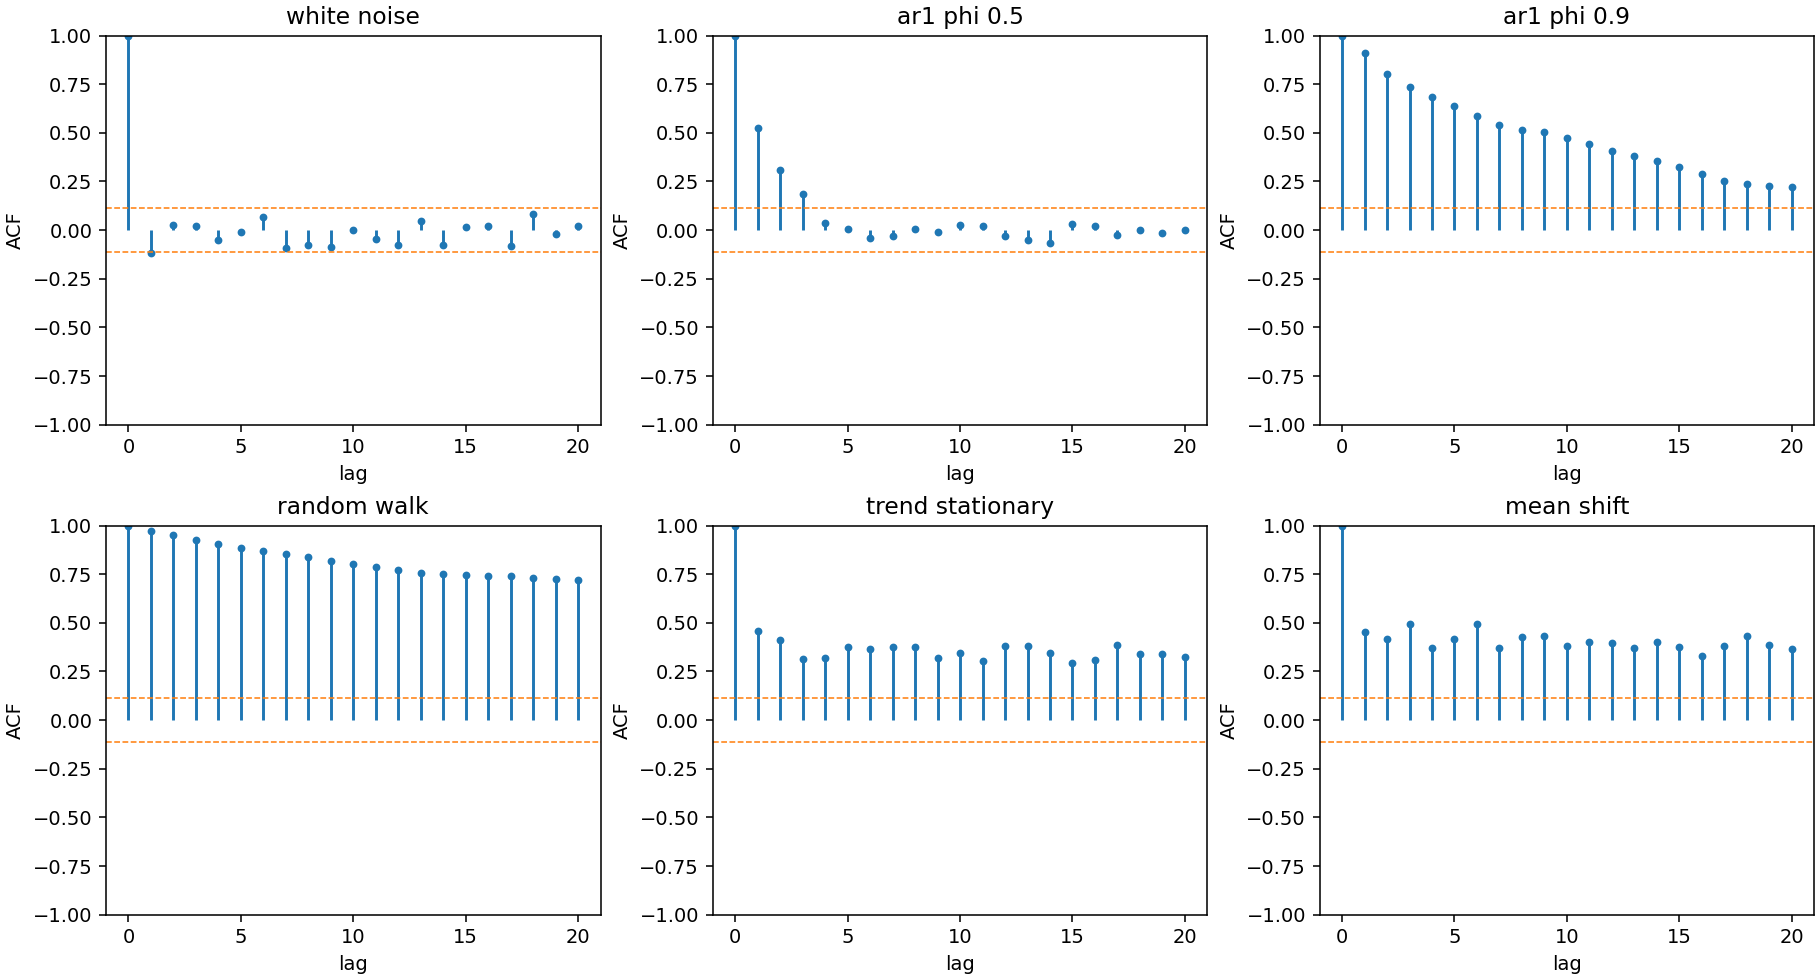
\includegraphics[width=0.94\textwidth]{../evidence/experiments/acf_diagnostics.png}
\caption{Sample autocorrelation profiles for the six generated processes. The artifact uses the fixed experiment configuration $n=300$, seed 20260910, and the associated 200-repetition study. AR(1) fitting and KPSS values produced by the broader script are exploratory and are not native APIs.}
\label{fig:acf-diagnostics}
\end{figure}

\subsection{Measured results}

Table~\ref{tab:diagnostics} reports the one-draw values. The white-noise result is compatible with weak sample autocorrelation, while the persistent AR(1) and random-walk draws show large positive lag-one ACF. Trend and midpoint-shift series also trigger the portmanteau statistic because the diagnostic responds to serial structure broadly; it does not identify its cause. The random-walk p-value stored as 0.0 is floating-point underflow, not an exact mathematical zero.

\begin{table}[htbp]
\centering
\caption{Single seeded draw for the three production diagnostics.}
\label{tab:diagnostics}
\begin{tabular}{@{}lrrrr@{}}
\toprule
Process & ACF(1) & $Q(20)$ & Ljung--Box $p$ & DW \\
\midrule
White noise & -0.1184 & 23.6152 & 0.2592 & 2.2325 \\
AR(1), $\phi=0.5$ & 0.4942 & 134.7573 & $6.8984\times10^{-18}$ & 1.0082 \\
AR(1), $\phi=0.9$ & 0.8707 & 749.5459 & $4.2036\times10^{-111}$ & 0.2499 \\
Random walk & 0.9796 & 4421.4050 & $0.0^{*}$ & 0.0086 \\
Trend plus noise & 0.3750 & 936.0809 & $3.7427\times10^{-136}$ & 0.5287 \\
Midpoint mean shift & 0.4854 & 1254.4266 & $1.2478\times10^{-176}$ & 0.7218 \\
\bottomrule
\end{tabular}
\vspace{0.25em}

\footnotesize $^{*}$Stored after floating-point underflow; not exact zero.
\end{table}

Across 200 repetitions, the 5\% Ljung--Box rejection rate is 0.065 for white noise and 1.000 for each of the other five generators. The white-noise rate is an empirical false-positive estimate. The other rates are detection frequencies for serial structure, not proof that all processes belong to one alternative model; only the two AR(1) generators are stationary AR alternatives. Monte Carlo error is material with 200 repetitions, and the synthetic length is short.

The broader experiment also computes an exploratory AR(1) fit/forecast and KPSS level/trend statistics. Those outputs are helpful research controls: the mean ACF(1) estimates are 0.4889 and 0.8827 for the two AR settings, and KPSS reacts to the random walk, trend, and shift according to its different stationarity null. However, they are intentionally excluded from Table~\ref{tab:diagnostics} and from the function count. KPSS uses interpolated asymptotic critical values, and the AR(1) routine is an external Python regression. Neither is implemented, registered, or benchmarked as a native aggregate. Likewise, the midpoint shift is a generated process, not a formal change-point test or location estimate.

\section{Benchmark evidence}

\subsection{Python state microbenchmark}

The benchmark compares two Python implementations. The \texttt{exact\_store\_sort} variant is the production-state model; \texttt{naive\_full\_recompute} is the baseline. Both retain rows and both finalizers compute actual ACF values through the requested lag, Ljung--Box $Q$, and Durbin--Watson. The benchmark separates add, merge, and finalize phases; combining numbers from different phases would be invalid. It explores 1,000, 5,000, and 10,000 rows; 128 random keys; lags 1, 8, and 64; 1, 4, and 16 chunks; contiguous and interleaved partitions; two repetitions; and seed 20260910.

\begin{table}[htbp]
\centering
\caption{Selected median Python timings for lag 64 and contiguous partitions.}
\label{tab:benchmark}
\begin{tabular}{@{}lrrrrrr@{}}
\toprule
Phase & Rows & Chunks & Exact ms & Naive ms & Exact bytes & Naive bytes \\
\midrule
Add & 1,000 & 1 & 0.339 & 0.137 & 135,236 & 129,285 \\
Merge & 5,000 & 16 & 0.444 & 0.193 & 617,056 & 645,249 \\
Finalize & 5,000 & 16 & 54.472 & 59.792 & 617,056 & 645,249 \\
Merge & 10,000 & 16 & 0.636 & 0.486 & 1,220,504 & 1,290,329 \\
Finalize & 10,000 & 16 & 157.828 & 179.847 & 1,220,504 & 1,290,329 \\
\bottomrule
\end{tabular}
\end{table}

The selected rows illustrate the intended complexity story without supporting a speedup claim. State bytes grow approximately linearly with row count. Merge is small because it is a sorted-vector operation after chunk construction, whereas finalization at lag 64 evaluates many lag products and dominates. In these selected cases the exact design finalizes faster than the naive baseline, but it adds and merges more slowly in several configurations. With only two repetitions, interpreter overhead, object layout, garbage collection, and timer noise are all important. The correct conclusion is that the measurement harness separates the relevant phases and confirms linear retained state; it does not predict native throughput.

The captured Python benchmark environment is CPython 3.12.6 on Windows 11 with 20 logical CPUs, and it records ClickHouse checkout commit \path{4d7f75efa83c3d81dff96373ce9874e2864c4e23}.

\subsection{Native ClickHouse measurements}

The native harness uses the linked ClickHouse 26.9.1.1 Debug binary on WSL2, Clang 21.1.8, an Intel Core i7-12700H, 20 logical CPUs, 7.6 GiB RAM, and \texttt{max\_threads=1}. Its deterministic signal is
\[
 x_t=\sin(0.017t)+0.25\cos(0.071t)+0.001(t\bmod 11).
\]
It evaluates all three functions for 1,000, 10,000, and 50,000 rows, with lag labels 1, 8, and 64, and three repetitions. Each timing launches a fresh \texttt{clickhouse local} process, evaluates the aggregate, and discards formatting with \texttt{FORMAT Null}. The visible warm-up row records ACF(8) 0.97338079, Ljung--Box $Q(8)$ 7856.153678662713, and Durbin--Watson 0.00059016.

\begin{table}[htbp]
\centering
\caption{Median native complete-process wall time at 50,000 rows.}
\label{tab:native-timing}
\begin{tabular}{@{}lrrr@{}}
\toprule
Function & Lag 1 & Lag 8 & Lag 64 \\
\midrule
Autocorrelation & 0.05 s & 0.06 s & 0.06 s \\
Ljung--Box & 0.05 s & 0.05 s & 0.06 s \\
Durbin--Watson control & 0.05 s & 0.05 s & 0.06 s \\
\bottomrule
\end{tabular}
\end{table}

Durbin--Watson has no lag parameter; its three labels repeat the same query as a matrix control. Median maximum resident set size across the largest cases is about 153 MiB, most of which is the ClickHouse process rather than the aggregate state. \texttt{/usr/bin/time} reports only hundredths of a second here, so startup dominates and the derived rows-per-second values are too coarse for a production claim.

\begin{table}[htbp]
\centering
\caption{Serialized autocorrelation states for 50,000 total samples.}
\label{tab:native-state-size}
\begin{tabular}{@{}rrr@{}}
\toprule
Partial states & RowBinary bytes & Construction time \\
\midrule
1 & 800,018 & 0.06 s \\
4 & 800,072 & 0.05 s \\
16 & 800,288 & 0.06 s \\
\bottomrule
\end{tabular}
\end{table}

These byte counts equal 16 bytes per retained \texttt{(UInt64, Float64)} sample plus an 18-byte version/cap/count header for each state. Merging 1, 4, or 16 partial states and aggregating the same 50,000 rows into 1, 4, or 16 series each records 0.05 s at this resolution. The raw 96 measurements, script, metadata, and summary are retained in the native-benchmark evidence. They confirm linear serialized storage and successful execution across the requested matrix; distinguishing algorithmic CPU constants requires a larger optimized-build study.

\section{Limitations and threats to validity}

The largest product limitation is memory. Exact arbitrary-order semantics retain one key/value record per accepted sample, so one high-cardinality group can use substantial arena memory and serialized storage. \texttt{max\_samples} makes the failure explicit but does not make the algorithm suitable for unlimited histories. Dirty states also require sorting, and Ljung--Box finalization costs $O(nH)$. Requesting every lag through $n-1$ would be quadratic; the hard lag cap limits configuration, not the fundamental cost.

The timestamp is an order key, not a sampling model. Gaps, unequal spacing, time zones, and calendar effects are not repaired. A position lag is meaningful only if the query's preprocessing gives positions a defensible interpretation. Duplicate timestamps fail instead of being averaged or selected. NULL rows are skipped by the engine, which can change spacing; users requiring explicit missing observations must regularize the series first.

Statistical interpretation is also limited. ACF is descriptive. Ljung--Box uses an asymptotic reference and depends on the chosen lag and any fitted-model degrees of freedom. Durbin--Watson is classically a regression-residual diagnostic, but this function accepts any supplied values and does not provide critical bounds or regression context. None of the three locates a change point, proves stationarity, fits an AR model, or generates a calibrated forecast.

Numerically, affine scaling and compensation reduce avoidable failures but do not remove \texttt{Float64} limits. Input conversion can round large integers, subnormal behavior is platform-dependent, and chi-square tail evaluation may underflow. Cross-platform checks should combine absolute and relative tolerance and separately assert finiteness, NaN contracts, and monotonic bounds such as $0\le p\le1$.

Finally, the empirical evidence is deliberately modest. Six synthetic generators, one length, one fixed seed, 200 repetitions, and a two-repeat Python benchmark cannot establish real-workload accuracy. Native validation uses a lean Debug build and one focused SQL test rather than the complete ClickHouse suite; the native timing matrix stops at 50,000 rows and is startup-limited. No release-mode or million-row throughput claim follows from it. These bounds define the evidence actually obtained rather than hiding unperformed work.

\section{Reproduction protocol}

From the manuscript directory, the independent reference, experiment, audit, and benchmark artifacts can be regenerated with the following commands:

\begin{lstlisting}[language={}]
py -3 -m unittest discover -s ../reference/python -p "test_*.py"
py -3 -m unittest discover -s ../evidence/experiments -p "test_*.py"
py -3 ../evidence/experiments/run_experiments.py --n 300 --reps 200 --seed 20260910 --output-dir ../evidence/experiments/results
py -3 ../evidence/experiments/audit_results.py --input-dir ../evidence/experiments/results --output ../evidence/experiments/results/analysis.md
py -3 ../evidence/benchmarks/benchmark_lag_state.py --output-dir ../evidence/benchmarks/reproduced --rows 1000,5000,10000 --lags 1,8,64 --chunks 1,4,16 --repeats 2 --seed 20260910
\end{lstlisting}

The generated \path{environment.json} files record the interpreter, packages, platform, seed, parameters, and source revision. Raw CSV files are retained alongside derived Markdown summaries. Native reproduction uses \path{research/REPRODUCING.md} and \path{build/run_native_validation.sh}; the latter creates a guarded temporary server configuration, runs a three-function local smoke, executes the focused SQL/Distributed fixture, and shuts the server down. From the repository root, the native benchmark command is:

\begin{lstlisting}[language={}]
REPEAT_COUNT=3 bash coursework/evidence/native-benchmark/run_native_benchmark.sh build-coursework/programs/clickhouse coursework/evidence/native-benchmark/reproduced
\end{lstlisting}

The completed native acceptance sequence built the aggregate and unified targets, ran the focused 15-test GoogleTest filter, started an isolated server, passed the stateless SQL pair including two logical shards, and then recorded the native benchmark. Compact outputs, environment, source hashes, binary hash, and build-log hashes are preserved under \path{evidence/native-validation/}; raw benchmark TSV files are preserved under \path{evidence/native-benchmark/}.

\section{Conclusion}

Ordered statistics expose a sharp boundary between a mathematical formula and a database aggregate. Autocorrelation, Ljung--Box, and Durbin--Watson are simple once one canonical series is available, but arbitrary parallel aggregation does not preserve that series unless the state does. A compact boundary envelope is not closed under interleaved merge trees; the $1,3,2$ counterexample makes the failure concrete. Retaining all keyed samples and merging their canonical union provides a direct associativity proof and a clear $O(n)$ resource contract.

The resulting coursework contribution is intentionally small and inspectable: exactly three APIs, one shared versioned state, explicit duplicate/non-finite/cap errors, scale-aware finalization, and layered evidence. Native evidence now includes warning-clean translation units, linked aggregate and unified targets, a three-function runtime smoke, 15/15 state tests, a passing SQL/Distributed fixture, and raw Debug benchmark measurements. The complete ClickHouse test corpus and release-performance study remain outside the claim. This restraint is also the central methodological result: aggregate functionality should be judged by its algebra, wire contract, test layers, and measured execution---not by the final statistical formula alone.

\bibliographystyle{plain}
\bibliography{../research/bibliography}

\end{document}
